%
% $RCSfile: architecture_context.tex,v $
%
% Copyright (c) 2001-2004. Christian Heller. All rights reserved.
%
% No copying, altering, distribution or any other actions concerning this
% document, except after explicit permission by the author!
% At some later point in time, this document is planned to be put under
% the GNU FDL license. For now, _everything_ is _restricted_ by the author.
%
% http://www.cybop.net
% - Cybernetics Oriented Programming -
%
% http://www.resmedicinae.org
% - Information in Medicine -
%
% @author Christian Heller <christian.heller@tuxtax.de>
%

\subsection{Architecture Context}
\label{architecture_context_heading}

To stepwise approach a solution, the problem needs to be placed in the right
context, that is the \emph{Physical} as well as \emph{Logical System Architecture}.

\begin{figure}[ht]
    \begin{center}
        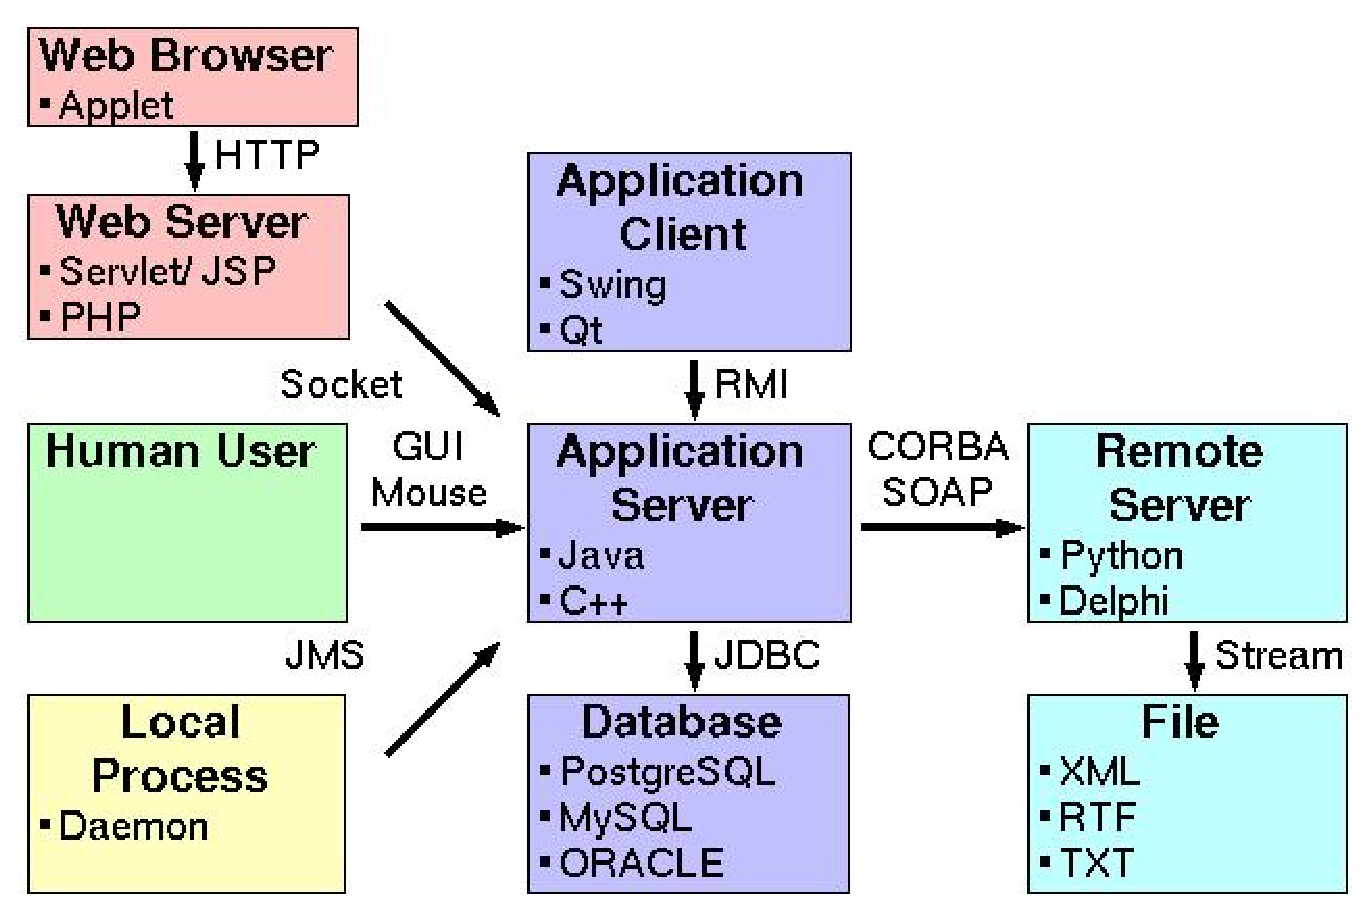
\includegraphics[scale=0.3]{vector/information_technology_environment.eps}
        \caption{Information Technology Environment}
        \label{information_technology_environment_figure}
    \end{center}
\end{figure}

Figure \ref{information_technology_environment_figure} shows a typical
\emph{Information Technology} (IT) environment (physical architecture).
There is a central \emph{Application Server} that is accessed by
\emph{Application Clients} or over \emph{Web}. In addition, it can be addressed
by \emph{Local Processes} (running on the same machine) and, most importantly,
\emph{Human Users} who control the system. The application server itself can
become a client by interacting with a \emph{Database System} or other
\emph{Remote Servers}.\\
Each of these kinds of communication makes use of its own interaction mechanism.
This paper will concentrate on the three (plus one) most important ones:
\begin{itemize}
    \item[-] Database (\emph{Backend})
    \item[-] Remote Server
    \item[-] Human User (\emph{Frontend})
    \item[-] Business Knowledge (\emph{Domain Model} in the Application Server itself)
\end{itemize}

A system to be capable of interacting via all of the above-mentioned kinds, needs to
have implemented the corresponding mechanisms in its software (logical architecture).
Figure \ref{inner_software_structure_figure} shows a possible inner software
structure of a modular (layered) system implementation.

\begin{figure}[ht]
    \begin{center}
        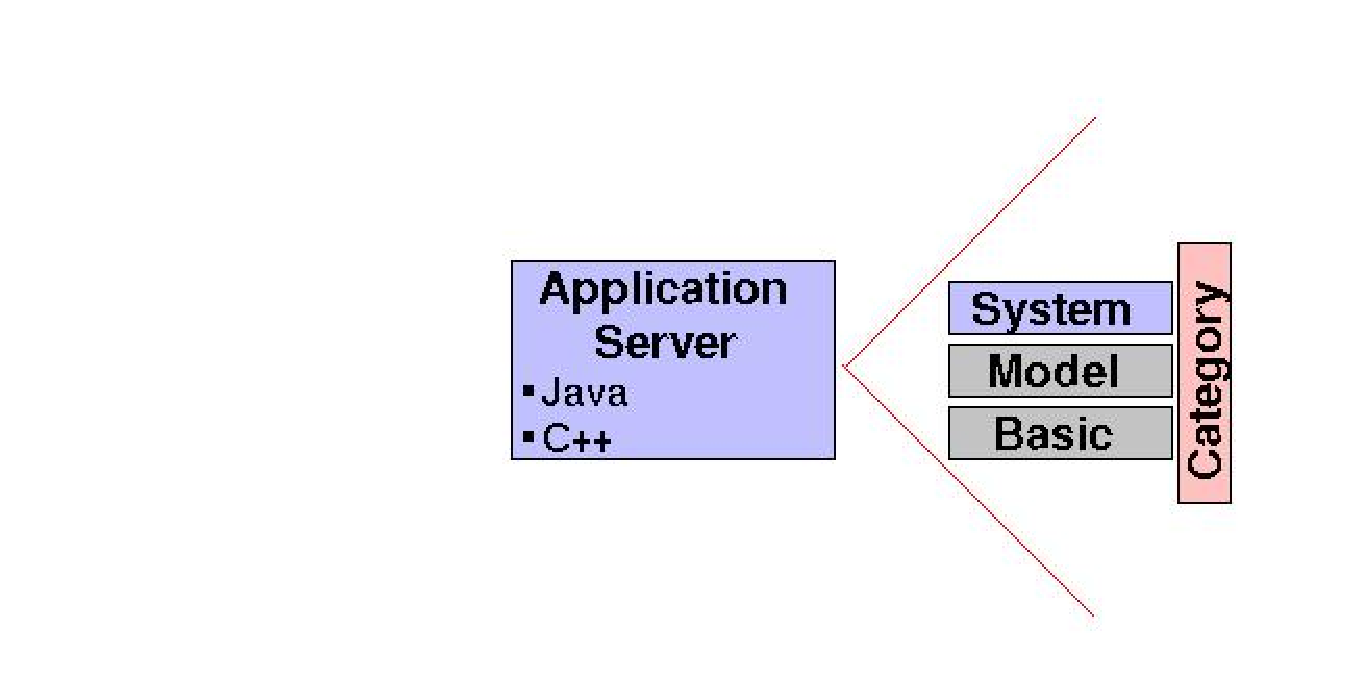
\includegraphics[scale=0.3]{vector/inner_software_structure.eps}
        \caption{Inner Software Structure}
        \label{inner_software_structure_figure}
    \end{center}
\end{figure}

